\chapter{Feasibility}
\section{Introduction}

\par
Our transportation application aims to enhance user experience by providing seamless navigation from the starting point to the destination. In addition to providing efficient routes, we also offer transparent pricing information, allowing users to select the transportation method that best suits their budget. Our navigator displays the actual cost of each route, enabling users to make informed decisions and pay only for the transportation they use. In addition, we provide the mini social media in the application, users can also share their recent transportation methods to the mini community so that other users can view them.
\section{Problem Statement}
\begin{figure}[!h]
    \centering
    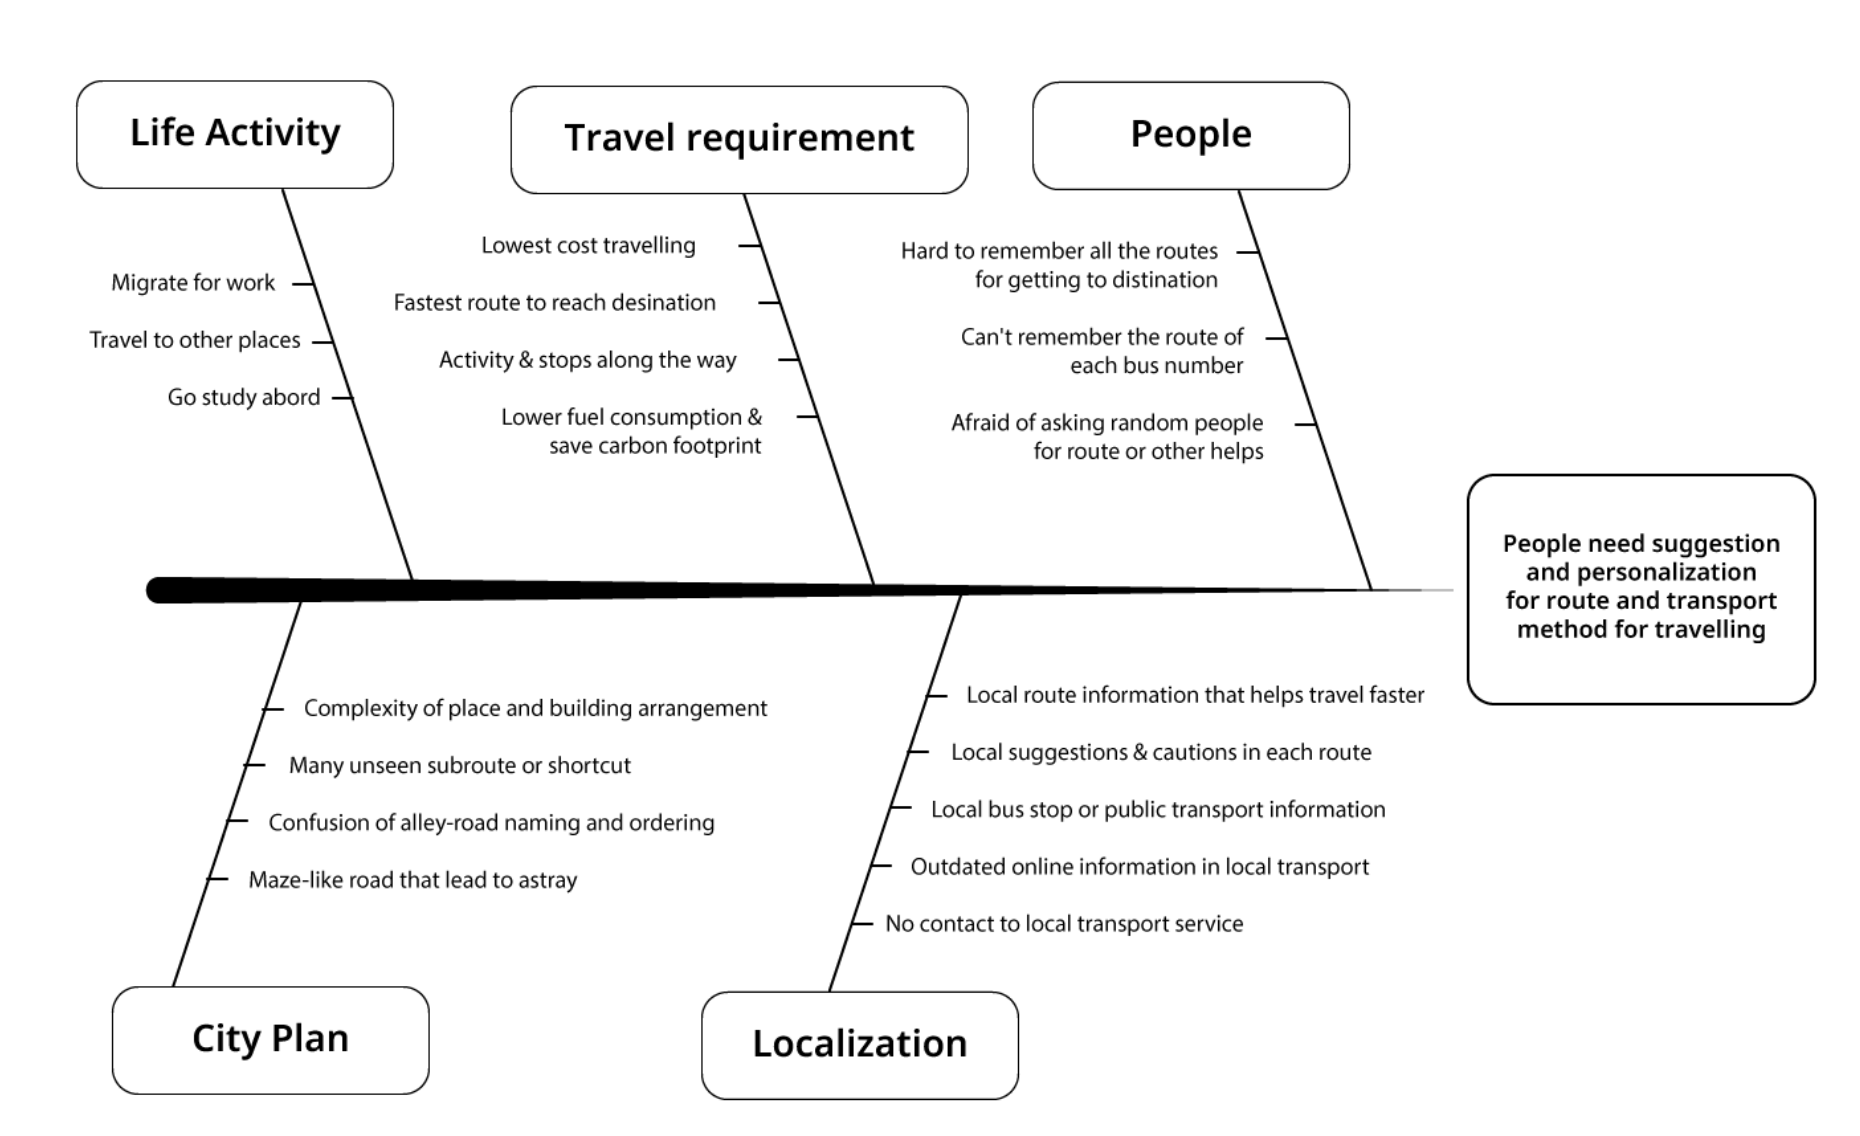
\includegraphics[width=0.8\linewidth]{chapter2/problem-statement.png}
    \caption{Problem diagram}    
    \label{fig:Problem diagram}
\end{figure}
\par
In people's everyday life, they need to transport to places for doing things, from daily commute to work, go on a trip or even going abroad. However, there's many concerning and obstacle for transportation. People themselves not able to remember all the routes (i.e., transportation line) that bring him to destination or sometimes there might be more better (in terms of cost, duration, or transfer) transportation route for them that they don't know. These problem may influenced by city plan that have complex arrangements or some localization that might leads to misinformation. As transportation, especially public transportation has a important impact to  people, improving transport information to be more accurate, accessible, and personalized will give an opportunity to people for more ease of life, so all these reasons lead to why we need a better routing application.

\newpage
\section{Related Research Projects}
\subsection{Google Maps}
This application is designed for regular users who use to find the location of the place, and transportation method between one point to another point, Google Maps allows users to see the detail of the traffic and estimate the time of transporting in each way that user select.
\begin{figure}[!h]
    \centering
    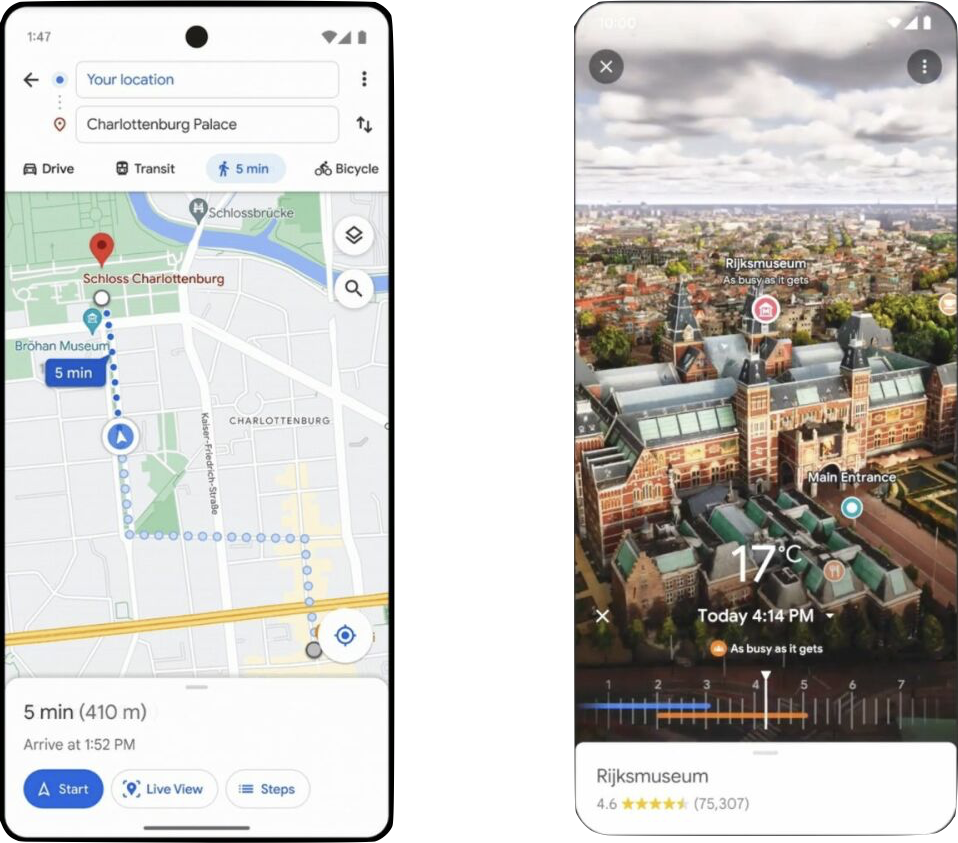
\includegraphics[width=0.5\linewidth]{chapter2/google_map.png}
    \caption{The Google Maps application}
    \label{fig:The Google Maps application}
\end{figure}

\subsection{Apple Maps}
This application is for Apple users that allows users to find the location, the way to go to their destination, estimate the time of transportation, see the details of traffic, and Apple Maps also provides the bicycle method, so cyclists can use Apple Maps to find the best way to get to their destination by bicycle.
\begin{figure}[!h]
    \centering
    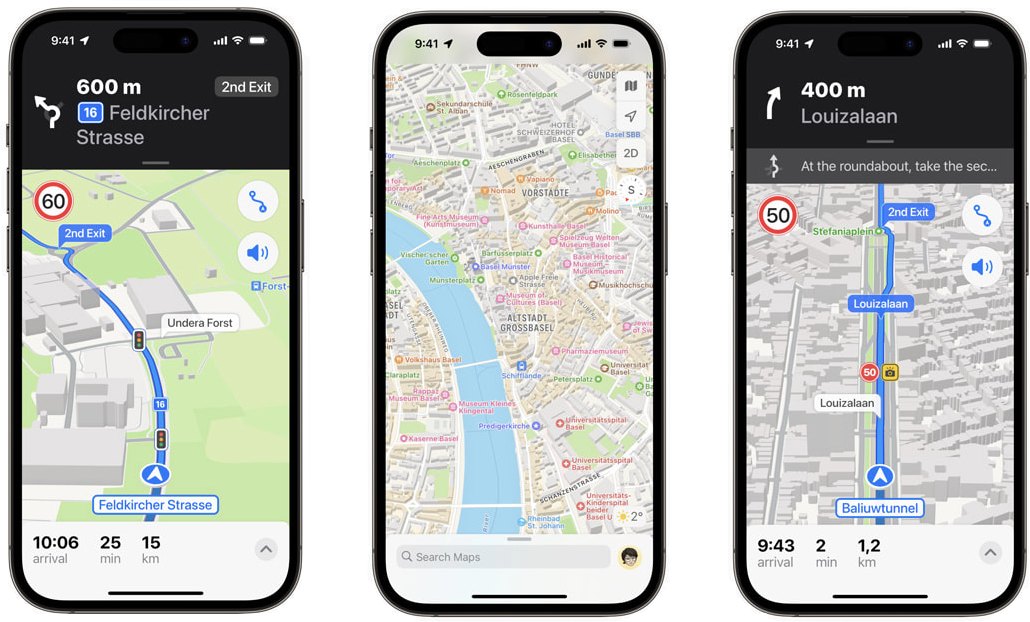
\includegraphics[width=0.5\linewidth]{chapter2/apple_map.png}
    \caption{The Apple Maps application}
    \label{fig:The Apple Maps application}
\end{figure}

\newpage
\subsection{ViaBus}
\par
ViaBus application is the application that provides user with the bus stops and routes, real-time bus locations approaching your stop, and recommended routes to travel from one place to another place which include buses, trains, and boats.
\begin{figure}[!h]
    \centering
    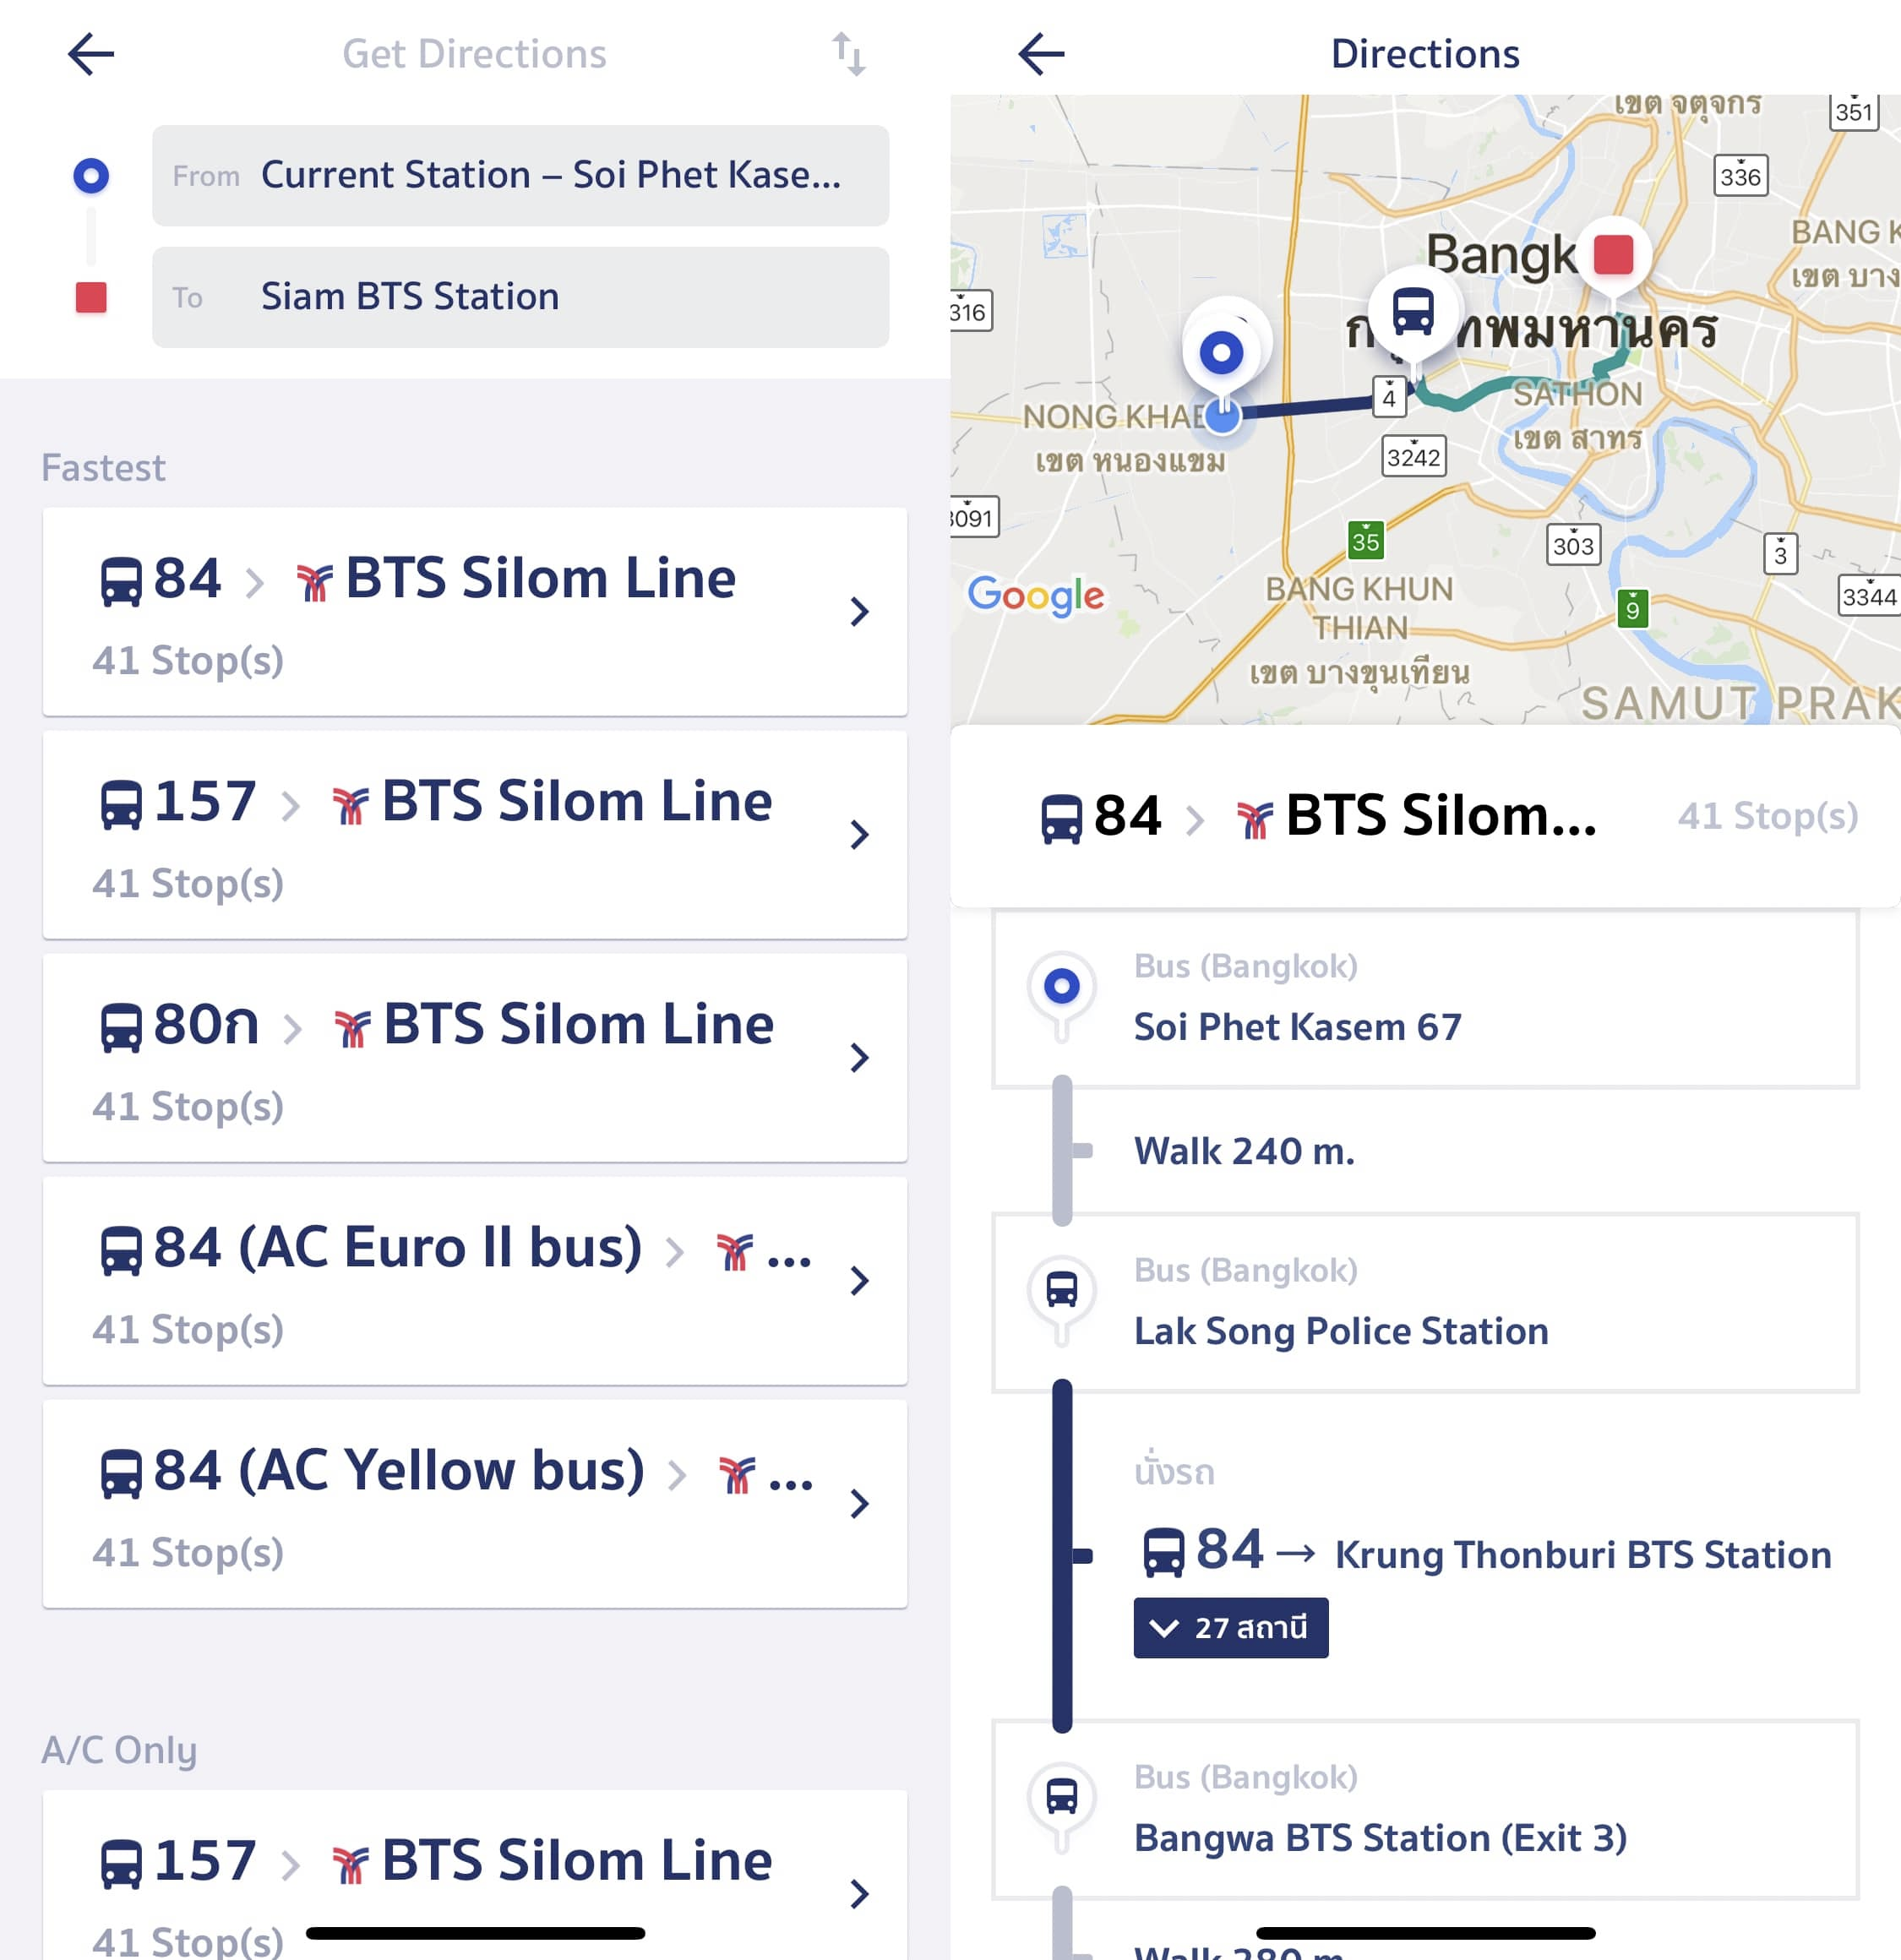
\includegraphics[width=0.5\linewidth]{chapter2/viabus.png}
    \caption{The ViaBus application}
    \label{fig:The ViaBus application}
\end{figure}

%---------------------------------------------------------------%
\subsection{Existing Functions}
\begin{table}[!h]
	\centering
	\resizebox{\linewidth}{!}{%
		\begin{tabular}{|>{\centering\hspace{0pt}}m{0.104\linewidth}|>{\centering\hspace{0pt}}m{0.085\linewidth}|>{\centering\hspace{0pt}}m{0.154\linewidth}|>{\centering\hspace{0pt}}m{0.173\linewidth}|>{\centering\hspace{0pt}}m{0.144\linewidth}|>{\centering\hspace{0pt}}m{0.142\linewidth}|>{\centering\arraybackslash\hspace{0pt}}m{0.129\linewidth}|} 
			\hline
			Applications & Map route & Search for destination & Routes recommendation & Estimate travel time & Estimate travel cost & Record travel info  \\ 
			\hline
			Google Maps  & Yes       & Yes                    & Yes                   & Yes                  & No                   & Yes                 \\ 
			\hline
			Apple Maps   & Yes       & Yes                    & Yes                   & Yes                  & No                   & Yes                 \\ 
			\hline
			ViaBus       & Yes       & Yes                    & No                    & No                   & No                   & No                  \\ 
			\hline
			TravelKit    & Yes       & Yes                    & Yes                   & Yes                  & Yes                  & Yes                 \\
			\hline
		\end{tabular}
	}
	\caption{Existing functions of related research application and TravelKit}
\end{table}

\newpage
\section{Requirement Specifications}
\subsection{System requirements}
\begin{itemize}
	\item Users select the destination after that the map view shows the path to travel to the destination, the estimated cost of traveling, and the estimated time to get there and the user can select the best way for them.
	\item Record the selected path from the user.
	\item Create the graph that provides the way to travel to the destination.
	\item Estimate the time from the one place to another place based on the path that is selected by the user.
	\item Estimate the cost on the selected path.
	\item Users can start and stop their trip.
	\item After a trip has been recorded, the application will record it in the database.
\end{itemize}

\subsection{Mobile application requirements}
\begin{itemize}
	\item Smartphone with Android OS or iOS
	\item Has geo-positioning sensor (GPS)
\end{itemize}

\section{Implementation Technique}
\begin{itemize}
	\item Frontend
	\begin{itemize}
		\item Programming language: Dart
		\item UI SDK: Flutter
		\item HTTP Client: Dio
	\end{itemize}
	\item Backend
		\begin{itemize}
		\item Go Runtime
		\item GoFiber for API server
	\end{itemize}
	\item Database Server
	\begin{itemize}
		\item MySQL: Persistent and relational data store
		\item MongoDB: Document Database for storing transport data
		\item Neo4j: Graph database for routing and path finding
	\end{itemize}
	\newpage
	\item 3rd party API
	\begin{itemize}
		\item Firebase Authentication: Sign-in and credential management
		\item Google Maps API: Geographic information retrieval
		\item OSRM: Routing engine for shortest paths in road networks
	\end{itemize}
	\item Infrastructure
	\begin{itemize}
		\item Container management: Docker
		\item DNS: Cloudflare
	\end{itemize}
	\item Development Software
	\begin{itemize}
		\item Visual Studio Code
		\item Goland
		\item DataGrip
		\item Postman
		\item iOS, Android simulator
	\end{itemize}
	\item Others
	\begin{itemize}
		\item Version Control: GitLab
		\item User interface design: Figma
	\end{itemize}
\end{itemize}

\section{Deliverables}
\subsection{Application}
\begin{itemize}
	\item Source code of application
	\item Mobile application
\end{itemize}
\subsection{Documentation}
	\begin{itemize}
	\item Project report
	\item Meeting log
	\item Poster
\end{itemize}

\newpage
\section{Implementation Plan}
\begin{figure}[!h]
	\centering
	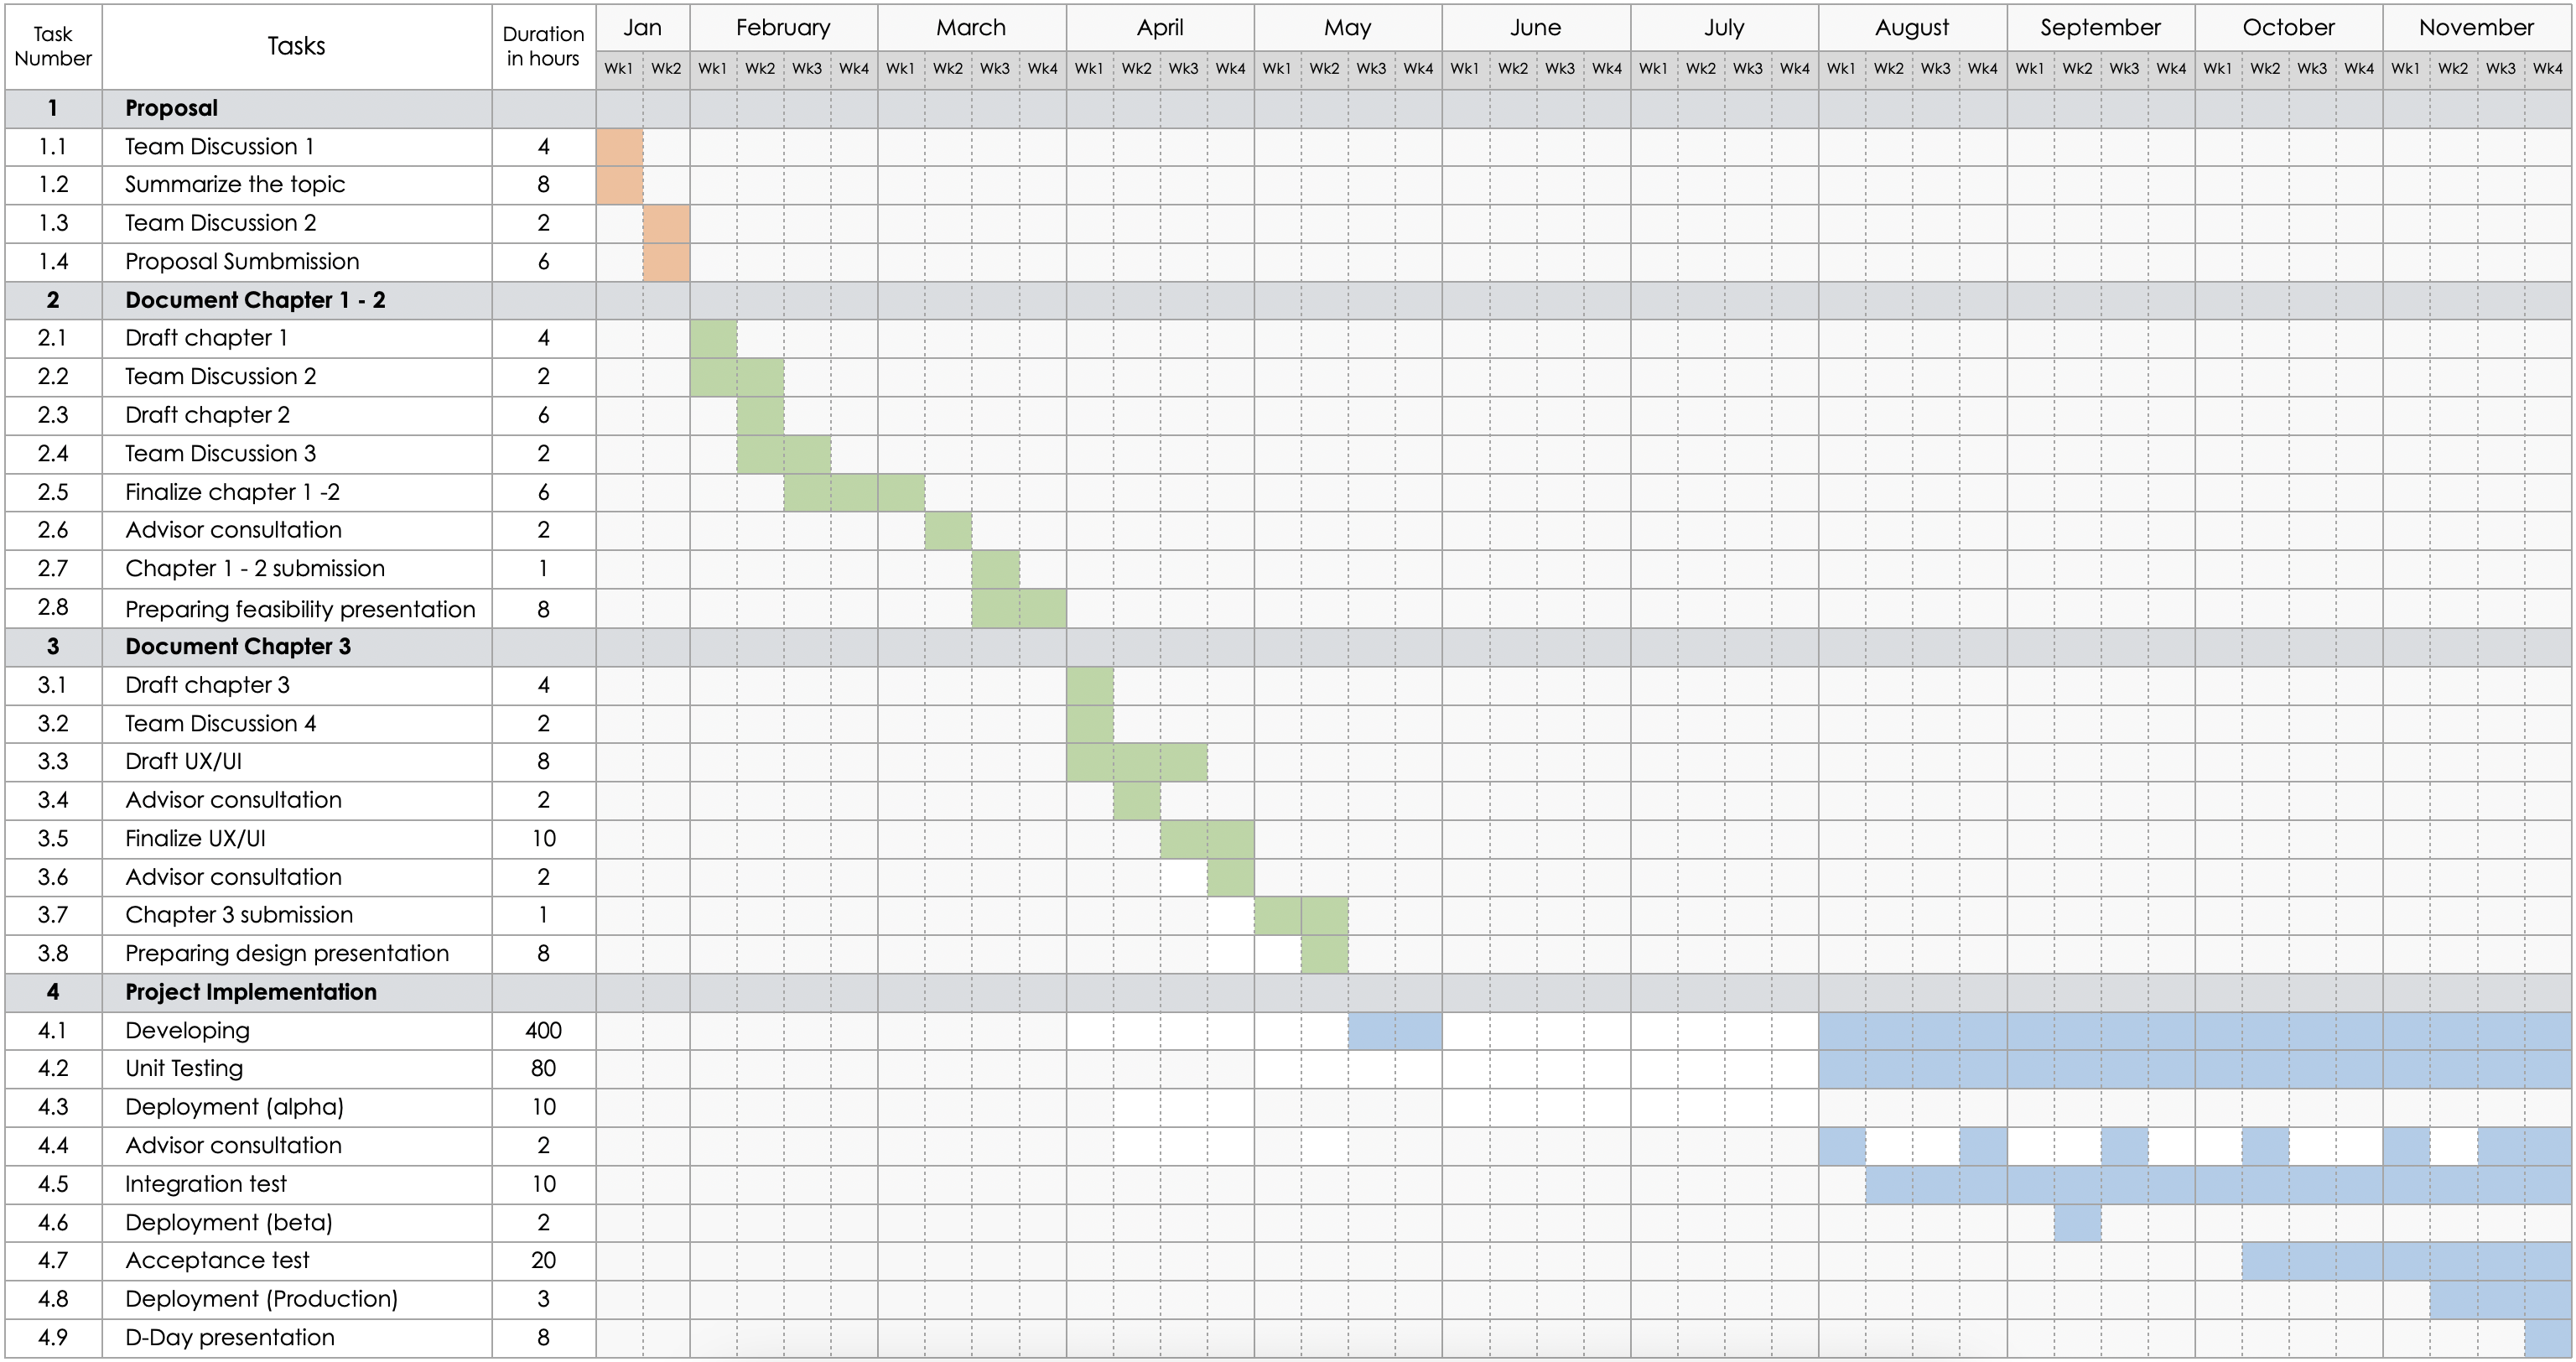
\includegraphics[width=1\linewidth]{chapter2/gantt_chart.png}
	\caption{Gantt Chart of the implementation plan}
	\label{fig:Gantt Chart of the implementation plan}
\end{figure}
\par
Our Implementation plan is divided into 4 phases that includes:
\begin{itemize}
	\item \textbf{Proposal Phase} During this initial stage, we engage in discussions to determine and finalize the topic for our project.
	\item \textbf{Document Chapter 1-2} In this phase, we delve into the conceptualization of ideas, feasibilities, conduct research, identify target users, and consult with advisors to gather essential information.
	\item \textbf{Document Chapter 3} This phase is dedicated to the creation of the project document, encompassing the development of diagrams, user personas, and the design of our application's user interface.
	\item \textbf{Project Implementation} The final phase involves a concentrated effort on coding, testing, and deploying our application.
\end{itemize}